\documentclass[14pt,a4paper]{article}
%\renewcommand{\baselinestretch}{1.5}
\linespread{1.3}
\usepackage[T2A]{fontenc} % Поддержка русских букв
\usepackage[utf8]{inputenc} 
\usepackage[english,russian]{babel}  
\bibliographystyle{unsrt}


\usepackage{graphicx}
\graphicspath{{imageWiMAX/}}
 
\begin{document}
\renewcommand\refname{Литература}
\thispagestyle{empty}

\begin{center}
\textbf{САНКТ-ПЕТЕРБУРГСКИЙ НАЦИОНАЛЬНЫЙ ИССЛЕДОВАТЕЛЬСКИЙ УНИВЕРСИТЕТ ИНФОРМАЦИОННЫХ ТЕХНОЛОГИЙ, 
МЕХАНИКИ И ОПТИКИ}

Факультет Компьютерных технологий и управления\\
Кафедра вычислительной техники
\end{center}
\vspace{2.5cm}

\begin{center}
\textbf{ОТЧЕТ}
\\
\textbf{о практике}

Исследование сетевых технологий с помощью имитационного моделирования
\end{center}

\vspace{2.5cm}

\begin{flushright}
\textbf{Студент}\\
Елькин А. А. группа 3105

\textbf{Руководитель практики}\\
Соснин В. В. доцент
\end{flushright}
\vspace{6cm}
\begin{center}
2014 год
\end{center}
%+++++++++++++++++++++++++++++++++++++++++++++++++++++++++++++++++++++++++++++++++++++++++++++++++++
%+++++++++++++++++++++++++++++++++++++++++++++++++++++++++++++++++++++++++++++++++++++++++++++++++++
%+++++++++++++++++++++++++++++++++++++++++++++++++++++++++++++++++++++++++++++++++++++++++++++++++++
%+++++++++++++++++++++++++++++++++++++++++++++++++++++++++++++++++++++++++++++++++++++++++++++++++++
%+++++++++++++++++++++++++++++++++++++++++++++++++++++++++++++++++++++++++++++++++++++++++++++++++++
\newpage
\tableofcontents
%+++++++++++++++++++++++++++++++++++++++++++++++++++++++++++++++++++++++++++++++++++++++++++++++++++
%+++++++++++++++++++++++++++++++++++++++++++++++++++++++++++++++++++++++++++++++++++++++++++++++++++
%+++++++++++++++++++++++++++++++++++++++++++++++++++++++++++++++++++++++++++++++++++++++++++++++++++
%+++++++++++++++++++++++++++++++++++++++++++++++++++++++++++++++++++++++++++++++++++++++++++++++++++
%+++++++++++++++++++++++++++++++++++++++++++++++++++++++++++++++++++++++++++++++++++++++++++++++++++
\newpage
\section{Система компьютерной верстки \TeX(\LaTeX)}
\subsection{\TeX}
\subsubsection{История \TeX}
\TeX{} \cite{wikiTeX:website} ~--- система компьютерной верстки, разработанная
Дональдом Кнутом, которая предназанчена для компьютерной верстки текста и математических формул. Кнут
начал разрабатывать систему в 1977 году, и первая версия \TeX{} вышла 1979
года. В 1982 году вышла заново переписанная версия \TeX'а, которой было дано
название TeX82. И с версии \TeX{} 3.0, которая получила лучшую поддержку
8-битных символов и различных языков, используеться нумирация: каждое обновление
добавляет в конец номера версии десятичную цифру так, что бы она приблежалась к
числу \begin{math} \pi \end{math}.

\subsubsection{Особенности \TeX}
В \TeX{} пользователь пишет тескст и задает лишь струкуту самого текста, а система
сама формирует документ на основе выбранного шаблона. Для задания структуры
используеться собственный язык разметки \TeX'а, все это содержиться в фалье с
расширением .tor, и \TeX{} транслирует в файл .dvi.

\TeX{} можно использовать для создания разных видов докуметов: книги, статьи,
отчеты, письма и др.

\subsection{\LaTeX}
\LaTeX{} \cite{wikiLaTeX:website}~--- макропакет компьютерной верстки \TeX{}. Он
не добаляет возможности в \TeX{}, а лишь позволяет автоматизировать задачи набора текста(умерация
разделов и формул, перекресные ссылки, размещение таблиц и т. п.). Первую версию
выпустил Лесли Лэмпортв 1984 году. В 1994 году была выпущена вторая версия
\LaTeX -- \LaTeXe{}, которая являеться текущей по сей день.

\subsection{Достоинства и недостатки \cite{Lvovskii}}
Среди достоинств можно выделить:
\begin{itemize}
\item{}Автор может не вникать в детали оформления документа, ему лишь надо
задать логическую структуру текста.
\item{}высокое качество и гибкость верстки абзацев и математических формул.
\item{}\TeX{} не требует большой вычеслительной мощности.
\item{}Система работает на большенства платформах.
\end{itemize}
Среди недостатков можно выделить:
\begin{itemize}
\item{}Исходный текст не будет выглядеть так же как при печати.
\item{}Создание нового макета документа очень трудоемкая задача.
\item{}\TeX{} плохо приспособлен для верстки страниц со сложным взаимодействие текста
и графиков.
\end{itemize}

\subsection{Список выбранного ПО}
Для написания отчета по практике был выбра ряд программного обеспечения:
\begin{enumerate}
\item Сборка \TeX'а MacTeX(http://tug.org/mactex/), включающий pdfLaTeX, который
выдает документ с расширение pdf.
\item IDE Eclipse(https://www.eclipse.org/) с расширением
TeXlipse(http://texlipse.sourceforge.net/), позволяющие удобно редактировать
документ.
\end{enumerate}
%+++++++++++++++++++++++++++++++++++++++++++++++++++++++++++++++++++++++++++++++++++++++++++++++++++
%+++++++++++++++++++++++++++++++++++++++++++++++++++++++++++++++++++++++++++++++++++++++++++++++++++
%+++++++++++++++++++++++++++++++++++++++++++++++++++++++++++++++++++++++++++++++++++++++++++++++++++
%+++++++++++++++++++++++++++++++++++++++++++++++++++++++++++++++++++++++++++++++++++++++++++++++++++
%+++++++++++++++++++++++++++++++++++++++++++++++++++++++++++++++++++++++++++++++++++++++++++++++++++
\newpage
\section{Система контроля верси Git}
\subsection{История Git}
Git \cite{wikiGit:website}~--- распределенная система контроля версиями.
Причиной создания Git послужило ухудшение отношейний между сообществом разработчиков Linux и компанией
разработавшей BitKeeper, используемым сообществом с 2002 года для разработки
Linux. Создателем проекта был Линус Торвальдс, и на сегодняшний день
поддердживаеться Джунио Хамано.
\subsection{Особенности Git}
В отличии от дугих СКВ Git не хранит изминения файлов, а сохраняет слепок файла
как она выгляид в данный момент, при чем, если файл не был изменен, он делает
ссылку на ранюю сохраненную версию файла. Так же большенство опраций с файлами
происходит локально, то есть для просмотра истории изменения проекта, создания
коммита можно не иметь доступа к Сети.

Git следит за целостностью данных, он вычисляет контрольную сумму(SHA-1 хеш),
которая становиться индексом данного файла. Данная система не позваляет изменять
содержимое файлов или каталога.
\subsection{Git-команды\cite{web:ProGit}}
\begin{enumerate}
  \item git help предаставляет список команд. Если использовать git
  --help <имя команды> даст справку об определенной команде.
  \item git init создает каталог .git со всей необходимой информацией о
  репозитории.
  \item git clone клонирует существующий репозиторий
  \item git remote отображает уже подключенные репозитории
  \item git remote add добавляет удаленный репозиторий
  \item git remote rm удаляет ссылку на репозиторий
  \item git add индексирует измененных файлом 
  \item git commit фиксирует измененные файлы
  \item git rm удаляет файлы
\end{enumerate}
Примеры ипользования приведенных команды находяться в каталоге "примеры Git
команд"
\newpage
\section{WiMAX}
WiMAX\cite{wikiWiMAX:website} ~--- телекоммуникационная технология,
предоставляющая универсальный беспроводной связи на большие расстояния для
разных устройств. Сеть WiMAX представляет собой совокунпность беспроводного
сегмента, который описываеться в стандарте IEEE 802.16, и базового сегмента, определенный
спецификациями WiMAX-форума\cite{WiMAXForum:website}.
\subsection{История WiMAX}
В декабре 2001 года была принята первая версия стандарта IEEE 802.16, который
описывал организацию широкоплосной беспроводной связи. Стандарт предусматривал 
скорость передачи информации 32-134 Мбит/с на расстояние в 2-5 км в радиоканалах
шириной 20, 25 и 28 МГц.

Из-за того, что была необходимо построение беспроводной сети только в зоне
прямой видимости, стандарт не получил широкого распространения. По этому в
январе 2003 года был принято расширение 802.15a, который изменял используемые
частоты на ча стоты в диапозоне от 2 до 11 ГГц. Это расширение должно было
обеспечивать скорость передачи информации 1-75 Мбит/с на теоретическое возможное
растояние 50км(в основном 6-9 км).

Стандарт IEEE 802.16e приняли в 2005 году. Он поддерживает мобильных абонентов и
систему роуминга между сетями различных беспроводных стандартов. 802.16e
позволял без разрыва сеанса переключаться между стандартами 802.11 и 802.16.

\subsection{Структура\cite{PathWiMAX} WiMAX}
Сеть состоит из двух основных подсистем: Access Service Network и Connectivity
Service Network.

CSN определяеться как набор функций для
абонента сети:
\begin{itemize}
\item{}Распределение адрессов между абонентами
\item{}Доступ к сети Интернет
\item{}Контроль доступа абонентов в сети
\item{}Биллинг и межаператорское взаимодествие
\item{}Обеспечение сервисов WiMAX
\item{}Обеспечение аутенфикации, авторизации и аудита соединения
\end{itemize}
ASN ~--- набор етевых элементов, организующие доступ в WiMAX сеть, выполняющие
функции:
\begin{itemize}
\item{}Доступ абонентов сеть по радиосвязи
\item{}Передача сообщений между CSN и абонентом для обеспечения аутенфикации,
авторизации и аудита соединения
\item{}Правление радиоресурсами
\item{}Поиск абонента в сети
\item{}Мобильность абонента
\end{itemize}
 
\begin{center}
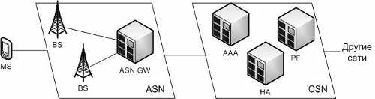
\includegraphics{WIMAX}
Структура сети WIMAX
\end{center}

\newpage
\addcontentsline{toc}{section}{Литература}
\bibliography{biblio}

\end{document}
 